
\section{Experimental Evaluation}
\label{sec:evaluation}
\label{sec:ramp-evaluation}

We proceed to experimentally demonstrate RAMP transaction scalability
as compared to existing transactional and non-transactional
mechanisms. \rapl, \rapb, and often \raps outperform existing
solutions across a range of workload conditions while exhibiting
overheads typically within $8\%$ and no more than $48\%$ of peak
throughput. As expected from our theoretical analysis, the performance
of our RAMP algorithms does not degrade substantially under contention
and scales linearly to over $7.1$ million operations per second on
$100$ servers. These outcomes validate our goal of coordination-free
design.

\subsection{Experimental Setup}
\label{sec:setup}

To demonstrate the effect of concurrency control on performance and
scalability, we implemented several concurrency control algorithms in
a partitioned, multi-versioned, main-memory database prototype. Our
prototype is in Java and employs a custom RPC system for
serialization. Servers are arranged as a distributed hash
table~\cite{chord} with partition placement determined by random
hashing of keys to servers. As in stores like Dynamo~\cite{dynamo},
clients can connect to any server to execute operations, which the
server will perform on their behalf (i.e., each server acts as a
client in our RAMP pseudocode). We implemented \rapl, \raps, and \rapb
and configure a wall-clock GC window of $5$ seconds as described in
Section~\ref{sec:additional}. \rapb uses a $256$-bit Bloom filter
based on an implementation of MurmurHash2.0~\cite{murmurhash}, with
four hashes per entry; to demonstrate the effects of filter
saturation, we do not modify these parameters in our experiments. Our
prototype utilizes the faster commit detection optimization from
Section~\ref{sec:additional}. We chose not to employ metadata garbage
collection and one-phase writes in order to preserve session
guarantees and because metadata overheads were generally minor.

\minihead{Algorithms for comparison} As a baseline, we do not employ
any concurrency control (denoted \nwnr, for no write and no read
locks); reads and writes take one RTT and are executed in parallel.

We also consider three lock-based mechanisms~\cite{gray-isolation}: long write locks and
long read locks, providing Repeatable Read
isolation (\textit{PL-2.99}; denoted \lwlr), long write locks with short read
locks, providing Read Committed isolation (\textit{PL-2L}; denoted
\lwsr; does not provide RA), and long write locks with no read locks,
providing Read Uncommitted isolation (\lwnr;
also does not provide RA). While only \lwlr provides RA, \lwsr and
\lwnr provide a useful basis for comparison, particularly in measuring
concurrency-related locking overheads. To avoid deadlocks, the system
lexicographically orders lock requests by item and performs them
sequentially. When locks are not used (as for reads in \lwnr and reads
and writes for \nwnr), the system parallelizes operations.

We also consider an algorithm where, for each transaction, designated
``coordinator'' servers enforce RA isolation---effectively, the Eiger
system's 2PC-PCI mechanism~\cite{eiger} (denoted \mstr;
Chapter~\ref{c.relatedwork}). Writes proceed via prepare and commit
rounds, but any reads that arrive at a partition and while a write
transaction to the same item is pending must contact a (randomly chosen,
per-write-transaction) ``coordinator'' partition to determine whether
the coordinator's prepared writes have been committed. Writes require
two RTTs, while reads require one RTT during quiescence and two RTTs
in the presence of concurrent updates (to a variable number of
coordinator partitions---linear in the number of concurrent writes to
the item). Using a coordinator violates partition independence
but---in this case---is still coordination-free. We optimize 2PC-PCI reads by having
clients determine a read timestamp for each transaction (eliminating
an RTT) and do not include happens-before metadata.

This range of lock-based strategies (\lwnr, \lwsr, \lwnr), recent
comparable approach (\mstr), and best-case (\nwnr; no concurrency
control) baseline provides a spectrum of strategies for comparison.

% espresso: 1000:1, f1 via spanner: 

\minihead{Environment and benchmark} We evaluate each algorithm using
the YCSB benchmark~\cite{ycsb} and deploy variably-sized sets of
servers on public cloud infrastructure. We employ \texttt{cr1.8xlarge}
instances on Amazon EC2 and, by default, deploy five partitions on
five servers. We group sets of reads and sets of writes into read-only
and write-only transactions (default size: 4 operations), and use the
default YCSB workload (\texttt{workloada}, with Zipfian distributed
item accesses) but with a 95\% read and 5\% write proportion, reflecting
read-heavy applications
(Section~\ref{sec:motivation},~\cite{tao,eiger,rainbird}; e.g., Tao's
500 to 1 reads-to-writes~\cite{tao,eiger}, Espresso's 1000 to 1
Mailbox application~\cite{espresso}, and Spanner's 3396 to 1
advertising application~\cite{spanner}).

By default, use $5000$ YCSB clients distributed across 5 separate EC2
instances. As in stock YCSB, each client makes a sequence of
synchronous requests to the database. When we later vary the number of
clients, we keep the number of servers hosting the clients fixed. To
fully expose our metadata overheads, use a value size of 1 byte per
write. We found that lock-based algorithms were highly inefficient for
YCSB's default 1000 item database, so we increased the database size
to one million items by default to decrease contention. Each version
contains a timestamp ($64$ bits), and, with YCSB keys (i.e., item IDs)
of size 11 bytes and a transaction length $L$, \rapl requires 11$L$
bytes of metadata per version, while \rapb requires 32 bytes. We
successively vary several parameters, including number of clients,
read proportion, transaction length, value size, database size, and
number of servers and report the average of three sixty-second trials.

\subsection{Experimental Results: Comparison}
\label{sec:eval-compare}

Our first set of experiments focuses on two metrics: performance
compared to baseline and performance compared to existing
techniques. The overhead of RAMP algorithms is typically less than
8\% compared to baseline (\nwnr) throughput, is sometimes zero, and
is never greater than 50\%. \rapl and \rapb always outperform the
lock-based and \mstr techniques, while \raps outperforms lock-based
techniques and often outperforms \mstr. We proceed to demonstrate this
behavior over a variety of conditions:



\minihead{Number of clients} RAMP performance scales well with
increased load and incurs little overhead
(Figure~\ref{fig:clients}). With few concurrent clients, there are few
concurrent updates and therefore few second-round reads; performance
for \rapl and \rapb is close to or even matches that of \nwnr. At peak
throughput with 10,000 clients, \rapl and \rapb pay a throughput
overhead of 4.2\% compared to \nwnr. \rapl and \rapb exhibit
near-identical performance; the \rapb Bloom filter triggers few false
positives and therefore few extra RTTs compared to \rapl. \raps
incurs greater overhead and peaks at almost 60\% of the throughput
of \nwnr. Its guaranteed two-round trip reads are expensive and it
acts as an effective lower bound on \rapl and \rapb performance. In
all configurations, the algorithms achieve low latency. \rapl, \rapb,
\nwnr less than 35~ms on average and less than 10~ms at 5,000
clients; \raps less than 53~ms, 14.3~ms at 5,000 clients.



In comparison, the remaining algorithms perform less favorably. In
contrast with the RAMP algorithms, \mstr servers must check a
coordinator server for each in-flight write transaction to determine
whether to reveal writes to clients. For modest load, the overhead of
these commit checks places \mstr performance between that of \raps and
\rapb.  Under YCSB's Zipfian workload, there is a high probability
that the several ``hot'' keys in the workload have a pending write,
requiring a \mstr commit check. The number of in-flight writes further
increases with load, increasing the number of \mstr commit
checks. This in turn decreases throughput, and, with 10,000 concurrent
clients, \mstr performs so many commit checks per read that it
underperforms the \lwnr lock-based scheme. Under this configuration,
more than 20\% of reads trigger a commit check, and, on servers with
hot items, each commit check requires indirected coordinator checks
for an average of 9.84 transactions. Meanwhile, multi-partition
locking is expensive~\cite{pavlo-partition}: with 10,000 clients, the
most efficient algorithm, \lwnr, attains only 28.6\% of the
throughput of \nwnr, while the least efficient, \lwlr, attains only
1.6\% and peaks at 3,412 transactions per second.


\begin{figure}[th!]
\begin{center}
{\includegraphics[width=\textwidth]{figs/legend-oneline.pdf}\vspace{0em}}
\includegraphics[width=.65\columnwidth]{figs/threads-thru.pdf}\vspace{-2em}
\includegraphics[width=.65\columnwidth]{figs/threads-lat.pdf}
\end{center}\vspace{-.5em}
\caption{Throughput and latency under varying client load. We omit
  latencies for \lwlr, which peaked at over 1.5s.}
\label{fig:clients}
\end{figure}


\begin{figure}[th!]
\begin{center}
\includegraphics[width=\textwidth]{figs/legend-oneline.pdf}\vspace{0em}
\includegraphics[width=.65\columnwidth]{figs/rprop-thru.pdf}\vspace{-1em}
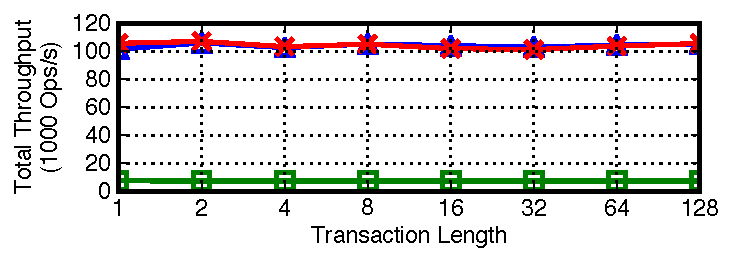
\includegraphics[width=.65\columnwidth]{figs/txnlen-thru.pdf}\vspace{-1em}
\includegraphics[width=.65\columnwidth]{figs/valuesize-thru.pdf}\vspace{-1em}
\includegraphics[width=.65\columnwidth]{figs/numkeys-thru.pdf}
\end{center}
\caption{Algorithm performance across varying workload
  conditions. \rapl and \rapb exhibit similar performance to \nwnr
  baseline, while \raps's 2 RTT reads incur a greater performance penalty
  across almost all configurations. RAMP transactions consistently
  outperform RA isolated alternatives.}
\label{fig:others}
\end{figure}

We subsequently varied several other workload parameters, which we
discuss below and plot in Figure~\ref{fig:others}:

\minihead{Read proportion} Increased write activity leads to a greater
number of races between reads and writes and therefore additional
second-round RTTs for \rapl and \rapb reads. With all write
transactions, all RAMP algorithms are equivalent (two RTT) and achieve
approximately 65\% of the throughput of \nwnr. With all reads, \rapl,
\raps, \nwnr, and \mstr are identical, with a single RTT. Between
these extremes, \rapl and \raps scale near-linearly with the write
proportion. In contrast, lock-based protocols fare poorly as
contention increases, while \mstr again incurs penalties due to commit
checks.


\minihead{Transaction length} Increased transaction lengths have
variable impact on the relative performance of RAMP
algorithms. Coordination-free execution ensures long-running
transactions are not penalized, but, with longer transactions,
metadata overheads increase. \rapl relative throughput decreases due
to additional metadata (linear in transaction length) and \rapb
relative performance also decreases as its Bloom filters
saturate. (However, YCSB's Zipfian-distributed access patterns result
in a non-linear relationship between length and throughput.) As
discussed above, we explicitly decided not to tune \rapb Bloom filter
size, but a logarithmic increase in filter size could improve \rapb
performance for large transaction lengths (e.g., 1024 bit filters
should lower the false positive rate for transactions of length 256
from over 92\% to slightly over 2\%).

\minihead{Value size} Value size similarly does not seriously impact
relative throughput. At a value size of 1B, \rapl is within 2.3\% of
\nwnr. However, at a value size of 100KB, \rapl performance nearly
matches that of \nwnr: the overhead due to metadata decreases, and
write request rates slow, decreasing concurrent writes (and
subsequently second-round RTTs). Nonetheless, absolute throughput
drops by a factor of 24 as value sizes moves from 1B to 100KB\@.

\minihead{Database size} RAMP algorithms are robust to high contention
for a small set of items: with only 1000 items in the database, \rapl
achieves throughput within 3.1\% of \nwnr. RAMP algorithms are
largely agnostic to read/write contention, although, with fewer items
in the database, the probability of races between readers and
in-progress writers increases, resulting in additional second-round
reads for \rapl and \rapb. In contrast, lock-based algorithms fare
poorly under high contention, while \mstr indirected commit checks
again incurred additional overhead. By relying on clients (rather than
additional partitions) to repair fractured writes, \rapl, \rapb, and
\raps performance is less affected by hot items. \vspace{.5em}

Overall, \rapl and \rapb exhibit performance close to that of no
concurrency control due to their independence properties and
guaranteed worst-case performance. As the proportion of writes
increases, an increasing proportion of \rapl and \rapb operations take
two RTTs and performance trends towards that of \raps, which provides
a constant two RTT overhead. In contrast, lock-based protocols perform
poorly under contention while \mstr triggers more commit checks than
\rapl and \rapb trigger second round reads (but still performs well
without contention and for particularly read-heavy workloads). The
ability to allow clients to independently verify read sets enables
good performance despite a range of (sometimes adverse) conditions
(e.g., high contention).


\begin{comment}
\begin{figure*}
\begin{center}
\includegraphics[width=.9\textwidth]{figs/legend-oneline.pdf}
\begin{minipage}[b]{0.49\linewidth}
\centering
\includegraphics[width=\textwidth]{figs/threads-thru.pdf}
\includegraphics[width=\textwidth]{figs/rprop-thru.pdf}
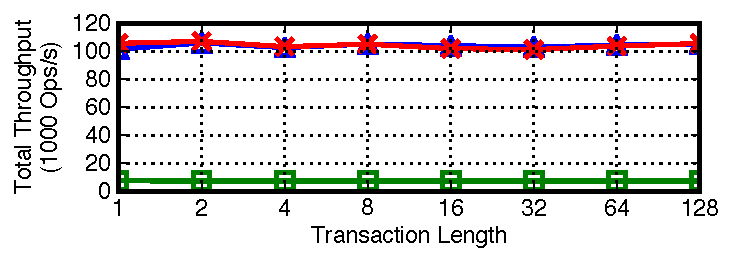
\includegraphics[width=\textwidth]{figs/txnlen-thru.pdf}
\includegraphics[width=\textwidth]{figs/valuesize-thru.pdf}
\includegraphics[width=\textwidth]{figs/numkeys-thru.pdf}
\end{minipage}
\begin{minipage}[b]{0.49\linewidth}
\centering
\includegraphics[width=\textwidth]{figs/threads-lat.pdf}
\includegraphics[width=\textwidth]{figs/rprop-lat.pdf}
\includegraphics[width=\textwidth]{figs/txnlen-lat.pdf}
\includegraphics[width=\textwidth]{figs/valuesize-lat.pdf}
\includegraphics[width=\textwidth]{figs/numkeys-lat.pdf}
\end{minipage}
\end{center}
\caption{Comparison of algorithms for default parameters, sweeping one
  parameter per experiment}
\label{fig:comparison}

\end{figure*}
\end{comment}

\FloatBarrier
\subsection{Experimental Results: CTP Overhead} 
\label{sec:ctp}

We also evaluated the overhead of blocked writes in our implementation
of the Cooperative Termination Protocol discussed in
Section~\ref{sec:replication}. To simulate blocked writes, we
artificially dropped a percentage of \textsc{commit} commands in
\textsc{put\_all} calls such that clients returned from writes early
and partitions were forced to complete the commit via CTP. This
behavior is worse than expected because ``blocked'' clients continue
to issue new operations. The table below reports the throughput
reduction as the proportion of blocked writes increases (compared to
no blocked writes) for a workload of 100\% \rapl write
transactions:
\begin{center}
\small 
\begin{tabular}{|l|c|c|c|c|}
\hline
\textbf{Blocked \%} & 0.01\% & 0.1\% & 25\% & 50\% \\\hline
{\textbf{Throughput}} & No change & 99.86\% & 77.53\% & 67.92\% \\\hline
\end{tabular}
\end{center}
As these results demonstrate, CTP can reduce throughput because each
commit check consumes resources (namely, network and CPU
capacity). However, CTP only performs commit checks in the event of
blocked writes (or time-outs; set to 5s in our experiments), so a modest
failure rate of $1$ in $1000$ writes has a limited effect. The higher
failure rates produce a near-linear throughput reduction but, in
practice, a blocking rate of even a few percent is likely indicative
of larger systemic failures. As Figure~\ref{fig:others} hints, the
effect of additional metadata for the participant list in \rapb and
\raps is limited, and, for our default workload of 5\% writes,
we observe similar trends but with throughput degradation of 10\% or
less across the above configurations. This validates our initial motivation
behind the choice of CTP: average-case overheads are small.

\subsection{Experimental Results: Scalability}



\begin{figure}[th!]
\begin{center}
\hspace{5mm}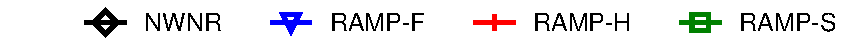
\includegraphics[width=\defaultfigwidth]{figs/legend-scaleout.pdf}\vspace{-.5em}
\includegraphics[width=.65\columnwidth]{figs/ns-thru.pdf}\vspace{-1.5em}
\includegraphics[width=.65\columnwidth]{figs/ns-perserver-thru.pdf}
\end{center}
\caption{RAMP transactions scale linearly to over $7$ million
  operations/s with comparable performance to \nwnr baseline.}
\label{fig:scaleout}
\end{figure}


We finally validate our chosen scalability criteria by demonstrating
linear scalability of RAMP transactions to 100 servers. We deployed an
increasing number of servers within the \texttt{us-west-2} EC2 region
and, to mitigate the effects of hot items during scaling, configured
uniform random access to items. We were unable to include more than 20
instances in an EC2 ``placement group,'' which guarantees 10 GbE
connections between instances, so, past 20 servers, servers
communicated over a degraded network. At around 40 servers, we
exhausted the \texttt{us-west-2b} ``availability zone'' (datacenter)
capacity and had to allocate our instances across the remaining zones,
further degrading network performance. To avoid bottlenecks on the
client, we deploy as many instances to host YCSB clients as we do to
host prototype servers.However, as shown in Figure~\ref{fig:scaleout},
each RAMP algorithm scales linearly. In expectation, at 100 servers,
almost all transactions span multiple servers: all but one in 100M
transactions is a multi-partition operation, highlighting the
importance of partition independence. With 100 servers, \rapl achieves
slightly under $7.1$ million operations per second, or 1.79 million
transactions per second on a set of 100 servers (71,635 operations
per partition per second). At all scales, \rapl throughput was always
within $10\%$ of \nwnr. With 100 servers, \rapl was within 2.6\%,
\raps within 3.4\%, and \raps was within 45\% of \nwnr. In light of
our scalability criteria, this behavior is unsurprising.

\FloatBarrier
